% ===========================================================================
% Chapter 9: Phase 2 proposal
% ===========================================================================
\chapter{Phase 2 Proposal}
\label{ch:phase2}

Phase~1 found that placement decides whether a candidate matters, but every run used one
weak description of vertical mixing (Chapter~\ref{ch:establish}). Phase~2
asks whether the verdict survives realistic transport and whether transport
can carry a candidate into the response band. It also takes up the detailed modelling of
ferric chloride, which the supervisor reserved for this phase.

% ===========================================================================
\section{The idea: fast winds, slow rising}
\label{sec:p2-idea}

The supervisor's direction, paraphrased: Venus rotates slowly, so its clouds are carried
round quickly while air rises slowly; if something from below reaches the cloud top and
absorbs ultraviolet light there, it should be looked for. A rough time for mixing to carry
a gas across a layer of thickness $L$ is $L^{2}/K_{zz}$, with $K_{zz}$ averaged over the
layer.

\begin{figure}[tbp]
  \centering
  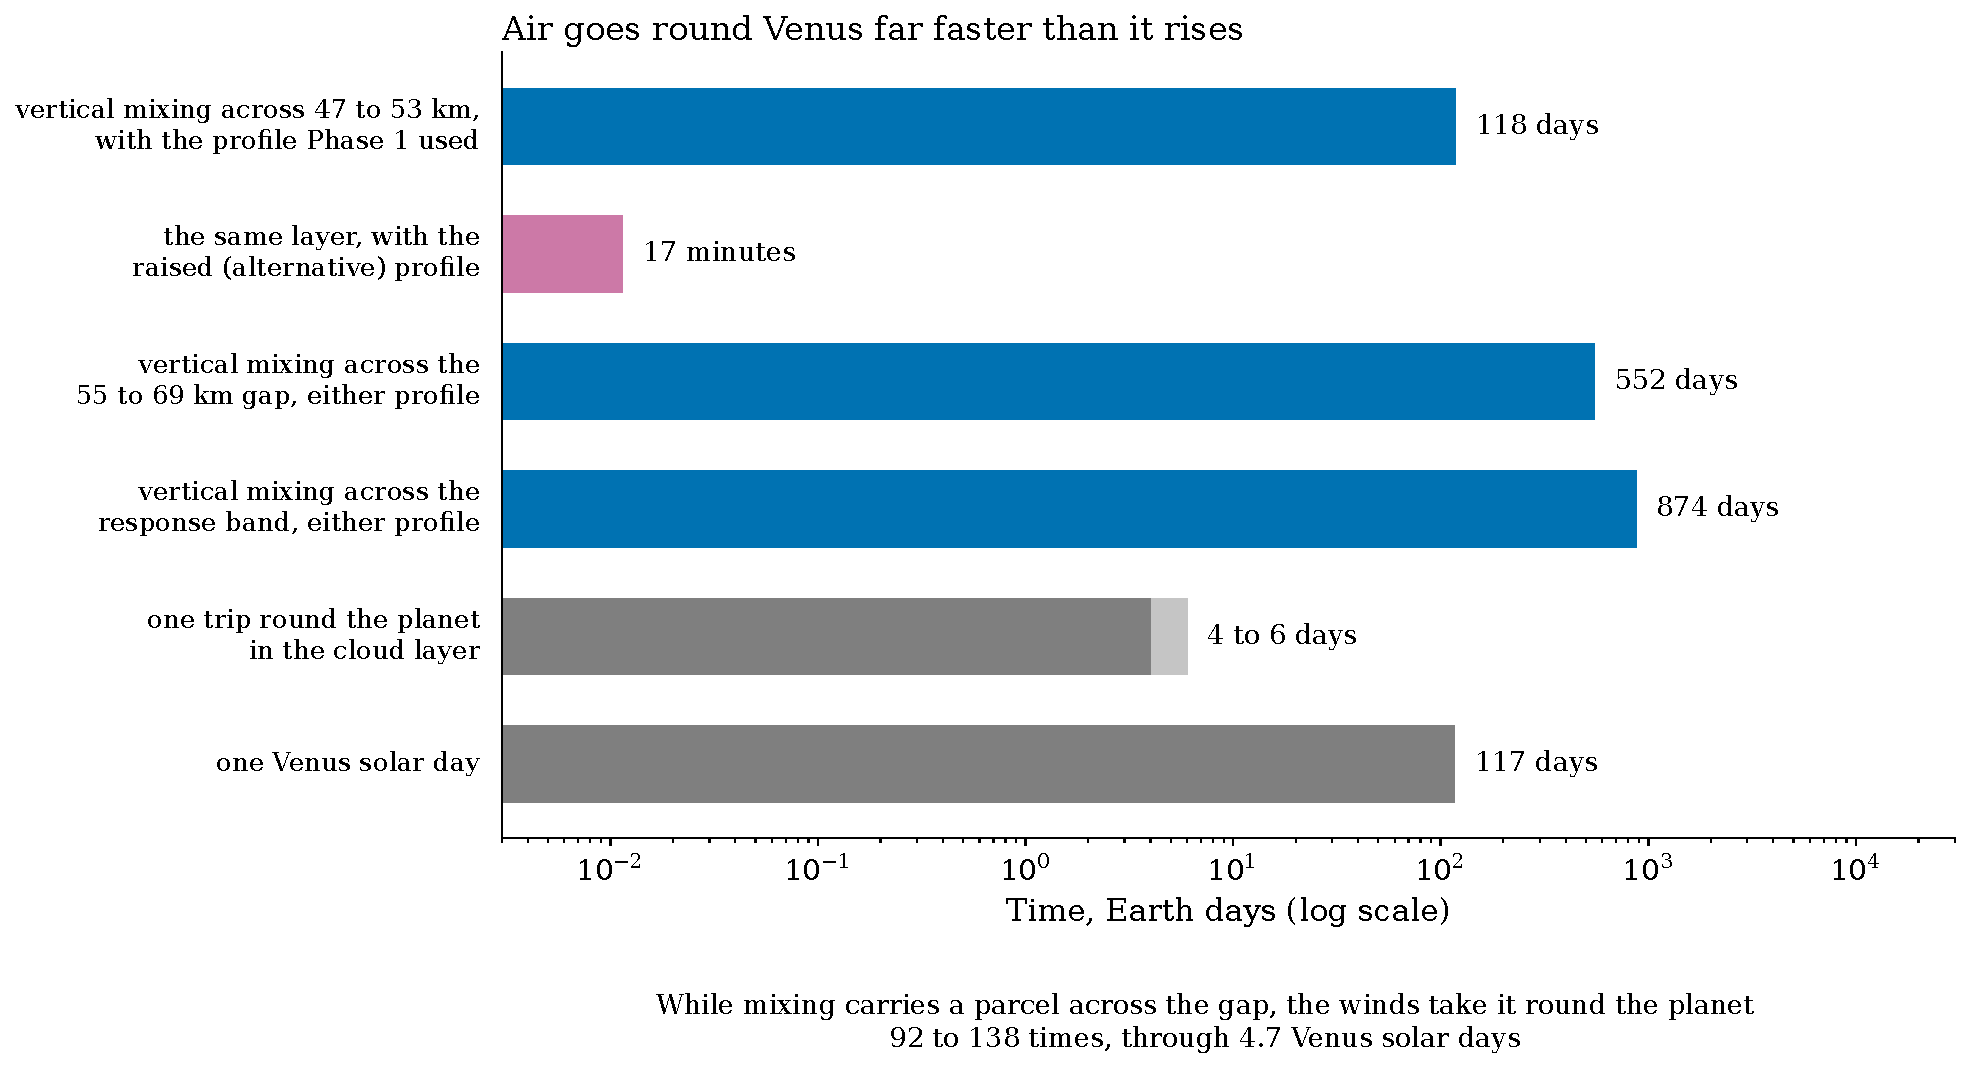
\includegraphics[width=0.7\textwidth]{F19_P2_transport-timescales_ch9_s19.pdf}
  \caption[Air goes round Venus far faster than it rises]{Air goes round Venus far faster than it rises. Mixing times $L^{2}/K_{zz}$
    across three layers, from the model's own mixing profiles, against the time for one
    trip round the planet~\cite{limaye2018} and one Venus solar
    day~\cite{bertaux2016}. Keys \texttt{p2.X.Bkzz.t\_days}, where X is the layer
    (\texttt{raised}, \texttt{gap} or \texttt{band}), and
    \texttt{p2.raised.BDkzz.t\_minutes}.}
  \label{fig:F19}
\end{figure}

Figure~\ref{fig:F19} shows the result. With the mixing profile of every Phase~1 run, a
gas needs about 552 days to cross the layer from 55 to 69~km (\texttt{p2.gap.Bkzz.t\_days})
and 874 days to cross the response band. The cloud layer goes round the planet in 4 to 6
days~\cite{limaye2018}, and one Venus solar day lasts 117 Earth
days~\cite{bertaux2016}. While mixing carries a parcel across the 55 to 69~km gap, the
winds take it round the planet 92 to 138 times, through 4.7 solar days. These times are
rough, but the contrast does not depend on the details.

% ===========================================================================
\section{What the literature adds}
\label{sec:p2-lit}

\textbf{The absorber is brought up, not made at the surface.} Bertaux et al.\ found that
the cloud-top wind and ultraviolet brightness at low southern latitudes vary with the
mountains of Aphrodite Terra below. Wind over the slopes launches gravity waves that
break just below the cloud top; where the wind speeds up, air must rise to make up for
it, and that upwelling brings the absorber to the cloud top. They also note that SO\sub{2}
falls from 150~ppmv at 54~km to 0.1 to 1~ppmv at the cloud top, so if the absorber comes
from SO\sub{2}, it ``must be produced inside the upper cloud, just below the cloud top
level''~\cite{bertaux2016}. The surface launches the waves; it does not supply the
molecule. Titov et al.\ tie the dark low-latitude markings to the same supply from
below~\cite{titov2008}.

\textbf{Mixing in the clouds is far stronger than Phase~1 assumed.} From Venus Express
sulfuric acid vapour, Dai et al.\ derived a global mean $K_{zz}$ peaking at
$5\times10^{8}$~cm$^{2}$\,s$^{-1}$ near 48~km and falling rapidly above
54~km~\cite{dai2023kzz}. Lef\`evre et al.\ found $10^{6}$ to $10^{8}$ in the 48 to 55~km
convective layer~\cite{lefevre2024}.

\textbf{A convective layer may sit inside the response band at noon.} In the model of
Lef\`evre et al., at the equator at noon, solar heating by the absorber itself drives a
convective layer at about 66 to 74~km, which the authors call still
speculative~\cite{lefevre2022}, overlapping the response band (Figure~\ref{fig:F20}). There,
a species whose chemical lifetime exceeds the 6000~s convective time becomes well
mixed~\cite{lefevre2022}. The authors note that the absorber's uncertain distribution ``could have a strong effect
on the cloud-top convection depth and vertical mixing'', and call for ``new 1D chemical
simulations with a more realistic convective mixing''~\cite{lefevre2022}. Phase~1 studied
exactly that distribution and its radiative effect.


\begin{figure}[tbp]
  \centering
  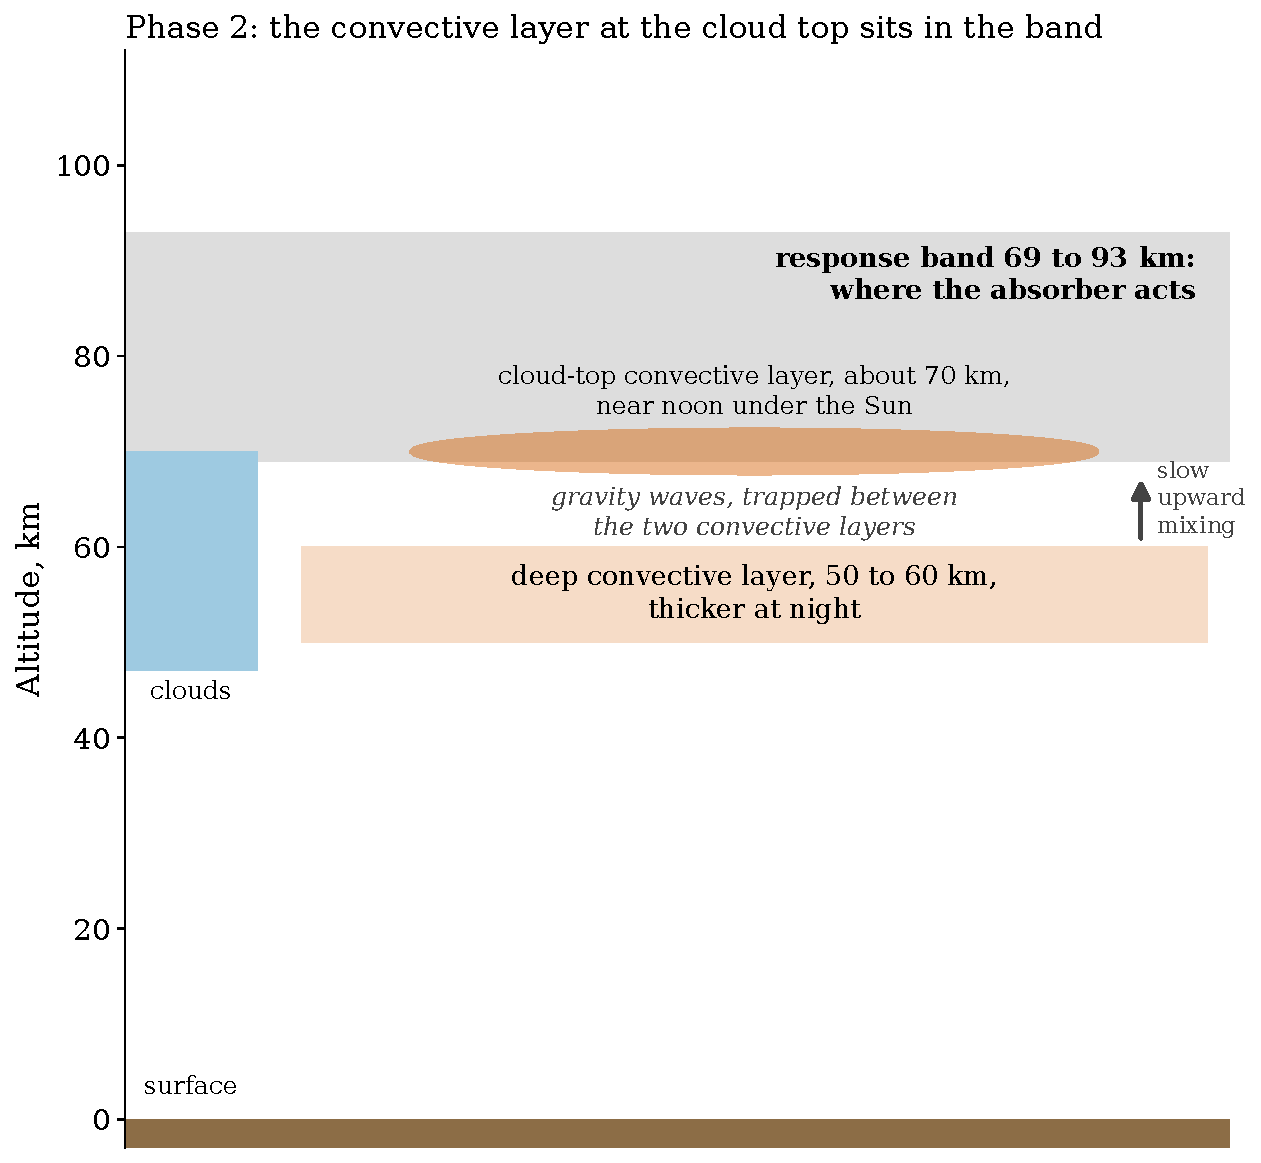
\includegraphics[width=0.7\textwidth]{F20_P2_altitude-map_ch9_s19.pdf}
  \caption[Where the layers sit]{Where the layers sit. The deep convective layer, 50 to 60~km in this study
    (other set-ups place it at 47 to 56 or 48 to 55~km, as above), is thicker at
    night; the cloud-top convective layer, near 70~km, appears at noon and lies inside
    the response band~\cite{lefevre2022}. Keys \texttt{e6.interval.90.lo} and
    \texttt{e6.interval.90.hi}.}
  \label{fig:F20}
\end{figure}

% ===========================================================================
\section{What the model already contains}
\label{sec:p2-model}

Three switches in the supplied code bear directly on Phase~2.

\textbf{A second mixing profile, never used.} The configuration file uses the mixing
in \texttt{atm/atm\_Venus\_Bkzz.txt}. A second file, named in a line that is commented
out, sits beside it: \texttt{atm/atm\_Venus\_B+Dkzz.txt}. The two are identical except at the four layers centred at
47 to 53~km, where the second is raised by 8716 to 14011 times
(\texttt{p2.kzz.raised.ratio\_min}, \texttt{.ratio\_max}) to the values of Dai et
al.~\cite{dai2023kzz} (Figure~\ref{fig:F18}). With it, the crossing time of that layer
falls from 118 days to 17 minutes. Every Phase~1 result was reached without this
enhancement. It stops at 53~km, so on its own it does not reach the band.

\begin{figure}[tbp]
  \centering
  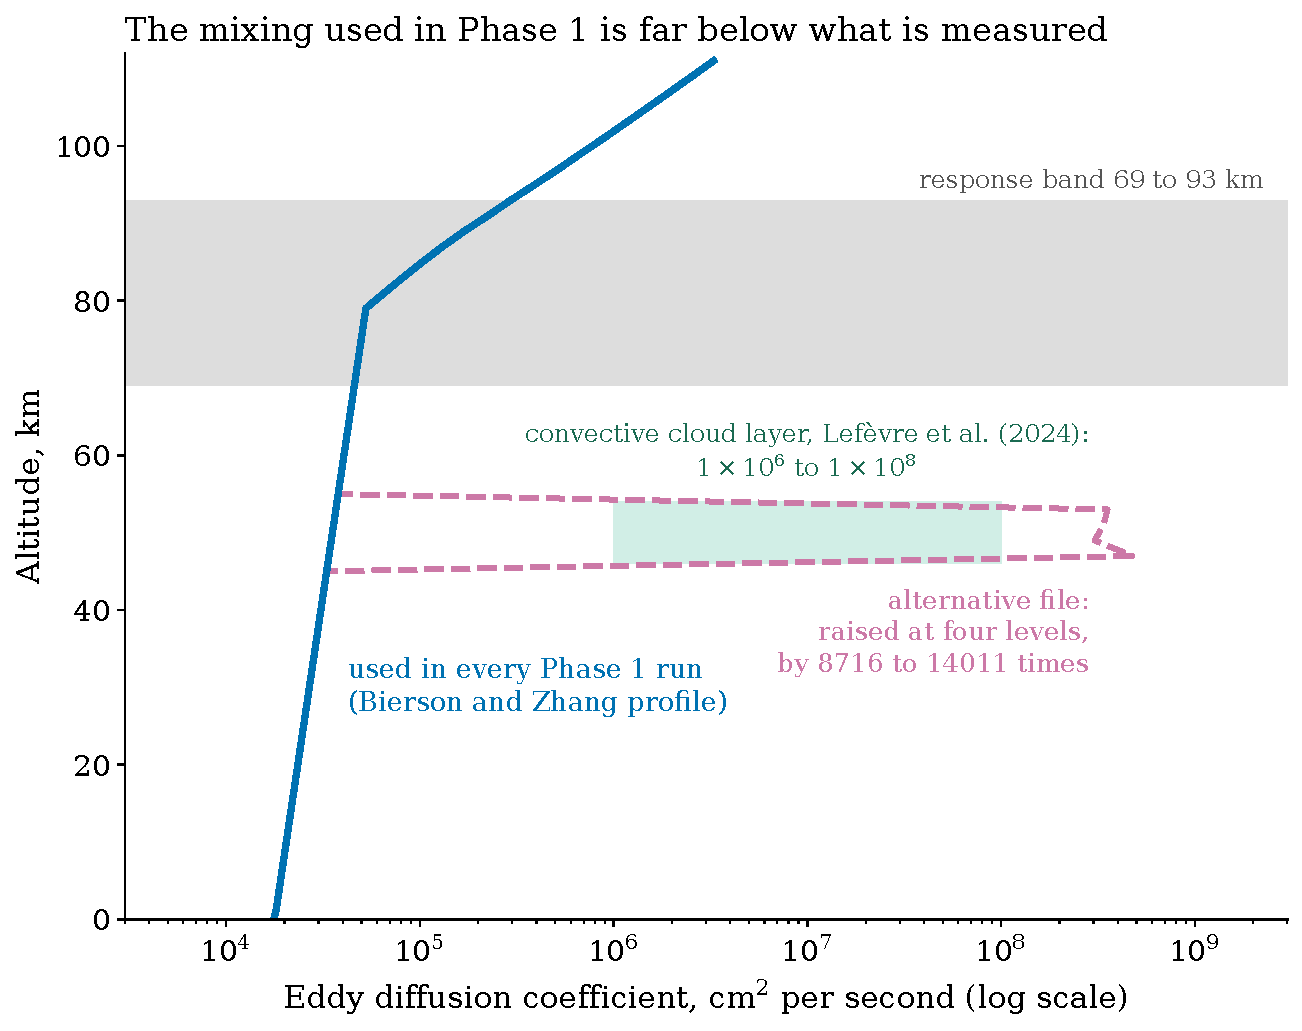
\includegraphics[width=0.7\textwidth]{F18_P2_two-mixing-profiles_ch9_report.pdf}
  \caption[The two mixing profiles supplied with the model]{The two mixing profiles supplied with the model. Solid: the profile of every
    Phase~1 run~\cite{bierson2020}. Dashed: the unused file, raised at four layers.
    Shaded: the convective layer of Lef\`evre et al.~\cite{lefevre2024}. Keys
    \texttt{p2.kzz.raised.ratio\_min} and \texttt{p2.kzz.raised.ratio\_max}.}
  \label{fig:F18}
\end{figure}


\textbf{Vertical wind, coded but off.} \texttt{use\_vz} is \texttt{False}, but upwind
advection is coded in \texttt{op.py}, and \texttt{build\_atm.py} can read a velocity per
level from a file.
\textbf{Day and night as two numbers.} Photolysis is halved (\texttt{f\_diurnal}) at one
zenith angle of 58 degrees (\texttt{sl\_angle}), untested for a noon-only layer.

% ===========================================================================
\section{Work packages}
\label{sec:p2-wp}

Each work package below is set out the same way: what changes in the model, what is
measured, what the result would mean, and what it needs first. Every measurement uses a
quantity Phase~1 already computes, so the registry and checker carry over unchanged.

\newpage
\textbf{WP1. Does the Phase~1 verdict survive stronger mixing?}
\nopagebreak[4]
\begin{itemize}[leftmargin=*, itemsep=1pt, topsep=2pt]
  \item \emph{Changes:} the mixing file named in \texttt{vulcan\_cfg.py}, switched to the
    raised profile of Section~\ref{sec:p2-model}; then a sweep of $K_{zz}$ from $10^{4}$
    to $10^{8}$~cm$^{2}$\,s$^{-1}$ over 46 to 70~km.
  \item \emph{Measures:} each candidate's centroid, its share of the column in the
    response band, and $\Delta F$ (Equation~\eqref{eq:field}), with the existing
    registry script.
  \item \emph{Would mean:} if the centroids and shares hold, the placement verdict
    survives the largest uncertainty in transport; if a candidate rises into the band,
    it goes back to the amount test. Dai et al.\ found the raised profile's effect on
    abundances ``slight''~\cite{dai2024}; the new question is placement and radiation.
  \item \emph{Needs:} nothing new; the file and the code exist.
\end{itemize}

\textbf{WP2. A cloud-top convective layer in one dimension.}
\nopagebreak[4]
\begin{itemize}[leftmargin=*, itemsep=1pt, topsep=2pt]
  \item \emph{Changes:} a new $K_{zz}$ profile that adds the noon layer near 70~km at
    the strength reported by Lef\`evre et al.~\cite{lefevre2022, lefevre2024}, justified
    against their published values.
  \item \emph{Measures:} the quantities of WP1, and the placement screen of
    Experiment~12 rerun on the new output.
  \item \emph{Would mean:} whether mixing inside the band can hold a candidate there.
    This is the piece that reaches into the band.
  \item \emph{Needs:} WP1, so that the effect of the new layer is separated from that of
    stronger mixing lower down.
\end{itemize}

\textbf{WP3. Upwelling.}
\nopagebreak[4]
\begin{itemize}[leftmargin=*, itemsep=1pt, topsep=2pt]
  \item \emph{Changes:} \texttt{use\_vz} switched on, with a vertical velocity for each
    level read from a file by \texttt{build\_atm.py} and used by the upwind advection
    already coded in \texttt{op.py}.
  \item \emph{Measures:} the inverse question: the smallest upward speed over 55 to
    67~km that delivers each candidate into the band before its chemistry destroys it.
  \item \emph{Would mean:} compared with what wave-driven upwelling could
    supply~\cite{bertaux2016}, whether rising air can do what mixing cannot. A
    one-dimensional model cannot represent a wave breaking over a mountain, so this
    tests a necessary condition only.
  \item \emph{Needs:} the lifetimes of WP5; it runs alongside WP2.
\end{itemize}

\textbf{WP4. The subsolar column.}
\nopagebreak[4]
\begin{itemize}[leftmargin=*, itemsep=1pt, topsep=2pt]
  \item \emph{Changes:} \texttt{sl\_angle} and \texttt{f\_diurnal} set for a column
    under the noon Sun instead of the halved, averaged sunlight, with a second column
    without sunlight for midnight, both on the mixing of WP2.
  \item \emph{Measures:} the quantities of WP1 at noon against the global mean, and
    SO\sub{2} at noon against the observed noon decrease of SO\sub{2} that accompanies an
    increase of the absorber~\cite{lefevre2022}.
  \item \emph{Would mean:} whether a candidate that fails in the global mean passes
    where light, heating and mixing are strongest together.
  \item \emph{Needs:} WP2.
\end{itemize}

\textbf{WP5. A fourth test: lifetime against transport.}
\nopagebreak[4]
\begin{itemize}[leftmargin=*, itemsep=1pt, topsep=2pt]
  \item \emph{Changes:} nothing in the model; a read-only script over saved output.
  \item \emph{Measures:} each candidate's chemical lifetime at each height, from its
    loss terms in \texttt{chem\_funs.py} read as in Experiment~5, against the time to
    reach the band, $L^{2}/K_{zz}$ (Section~\ref{sec:p2-idea}), with the 6000~s
    convective time at 70~km~\cite{lefevre2022} as a mark.
  \item \emph{Would mean:} a fourth axis for the screen of Experiment~12, and the answer
    to why the chemistry keeps ClS\sub{2} low (Experiment~9).
  \item \emph{Needs:} the output of WP1.
\end{itemize}

\textbf{WP6. Ferric chloride.}
\nopagebreak[4]
\begin{itemize}[leftmargin=*, itemsep=1pt, topsep=2pt]
  \item \emph{Changes:} iron and chlorine chemistry added to the network (a meteoric
    iron source, reactions with hydrogen chloride, uptake into droplets), and the
    ferric chloride cross sections obtained from the laboratory group.
  \item \emph{Measures:} the placement test of Experiment~9 for ferric chloride: its
    centroid, its share in the band and $\Delta F$.
  \item \emph{Would mean:} whether ferric chloride sits where the absorber acts, the
    test that Experiment~14 could not make.
  \item \emph{Needs:} the transport framework of WP1 to WP4; some rate constants may not
    exist, which is why it comes last.
\end{itemize}

\textbf{Order and risks.} WP1 and WP5 come first and can give a publishable result on
their own; WP2 and then WP4 follow, WP3 alongside WP2, and WP6 last. Three risks are
stated now. The absorber's heating drives the mixing that would move it, so the test will
be run with the mixing that heating would give and without it, and both reported. The
ferric chloride preprint's group is active~\cite{egan2026}, so WP6 may be overtaken. And
the 55 to 69~km gap may prove uncrossable; if so, that is the result.
